\uuid{KSv1}
\exo7id{7287}
\auteur{mourougane}
\organisation{exo7}
\datecreate{2021-08-10}
\isIndication{false}
\isCorrection{false}
\chapitre{Géométrie affine euclidienne}
\sousChapitre{Géométrie affine euclidienne du plan}

\contenu{
\texte{
\label{inter-droites-compas-seul}
On considère quatre points distincts \(A\), \(B\), \(C\), \(D\), 
tels que les droites \((AB)\) et \((CD)\) soient sécantes en un point \(X\). 
On veut construire le point \(X\) au compas seul.

\begin{center}
    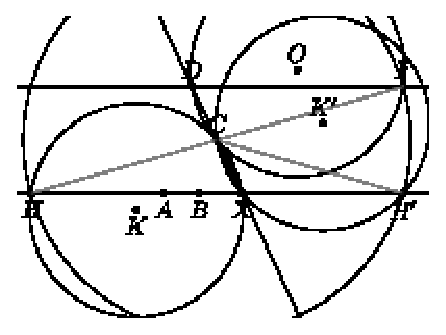
\includegraphics[scale=1]{images/img-mour-039}
\end{center}

% [[figure asymptote]]

%\begin{center}
%\begin{asy}
%size(7cm, 0);
%point A = (0, 0); dot("\(A\)", A, S);
%point B = (1, 0); dot("\(B\)", B, S);
%line L0 = line(A, B); draw(L0);
%point C = (1.5, 1.5); dot("\(C\)", C, N);
%point D = (0.8, 3); dot("\(D\)", D, N);
%line L1 = line(C, D); draw(L1);
%point X = intersectionpoint(L0, L1); dot("\(X\)", X, S);
%line L2 = parallel(D, L0); draw(L2);
%real r = 3;
%point O = intersectionpoints(circle(C, r), circle(D, r))[1];
%dot("\(O\)", O, N);
%circle C0 = circle(O, r); clipdraw(C0);
%point[] DF = intersectionpoints(C0, L2);
%point F = (DF[0] == D) ? DF[1] : DF[0]; dot("\(F\)", F, N);
%circle C1 = circle(C, abs(F - C)); clipdraw(C1);
%point[] H = intersectionpoints(C1, L0);
%dot("\(H\)", H[0], S); dot("\(H'\)", H[1], S);
%draw(C--F, gray); draw(C--H[0], gray); draw(C--H[1], gray);
%point K0 = intersectionpoints(circle(C, r), circle(H[0], r))[0];
%point K1 = intersectionpoints(circle(C, r), circle(H[1], r))[1];
%dot("\(K\)", K0, S); dot("\(K'\)", K1, N);
%circle C2 = circle(K0, r); draw(C2);
%circle C3 = circle(K1, r); draw(C3);
%\end{asy}
%\end{center}
}
\begin{enumerate}
    \item \question{À l'aide de l'exercice~\ref{para-compas-seul}, expliquer comment 
construire la parallèle \( \Delta\) à \((AB)\) passant par \(D\).}
    \item \question{Construire un point \(O\) équidistant de \(C\) et \(D\), et \(F\) 
le point d'intersection du cercle de centre \(O\) passant par \(C\) et \(D\) 
avec ma droite \( \Delta\), autre que \(D\). On note \(H\) et \(H'\) les points 
d'intersection du cercle de centre \(C\) passant par \(F\) avec la 
droite \((AB)\). Comment construire ces points au compas seul?}
    \item \question{Construire le centre \(K\) de \(\mathcal{C}\), un des deux cercles 
de rayon \(OC\) passant par \(C\) et \(H\). De même, construire le centre \(K'\) 
de \(\mathcal{C}'\), un des deux cercles de rayon \(OC\) passant par \(C\) 
et \(H'\). Montrer que le point \(C\) est commun à \(\mathcal{C}\) 
et \(\mathcal{C}'\).}
    \item \question{Notons \( \alpha\) la mesure de l'angle \(\widehat{AXD}\). En supposant que 
les points sont disposés comme sur la figure ci-dessus, montrer que:
\begin{enumerate}}
    \item \question{la mesure de \(\widehat{CDF}\) est \( \alpha\);}
    \item \question{la mesure de \(\widehat{COF}\) est \(2 \alpha\);}
    \item \question{la mesure de \(\widehat{CKH}\) est \(2 \alpha\);}
    \item \question{la mesure de \(\widehat{CK'H'}\) est \(2 \alpha\).}
\end{enumerate}
}
